% Introduction to additive manufacturing >>>
Additive manufacturing (AM) is described in ISO/ASTM 52900 \cite{organization_isoastm_2015} as the "process of joining materials to make parts from 3D model data, usually layer upon layer, as opposed to subtractive manufacturing and formative manufacturing methodologies".
In this first chapter, we will discuss and describe AM processes or, popularly, 3D printing processes, which will most likely characterize the manufacturing scenario in upcoming years. From the 1950s - 1960s, before being called AM processes, these processes were called "Rapid Prototyping" (RP). From the name, it is easy to understand why these technologies were first developed: a lean approach to new product development process would allow cost and time-to-market reduction. Only in 1984 and 1986 the first 3D printing technologies were patented, and the possibility of manufacturing a finished object by adding material layer by layer became a reality. The early 2000s were characterized by a push towards using these technologies also for large-scale production. Indeed, the first cost studies associated with 3D printing usage for mass production were conducted in these years, among which it's worth mentioning the one from \citeauthor{hopkinson_analysis_2003} (2003). According to the authors, for small production batches, AM technologies were more cost-effective and achieved a quality sufficient to ensure the products were saleable (Fig. \ref{fig:costs}).
\begin{figure}[H]
    \centering
    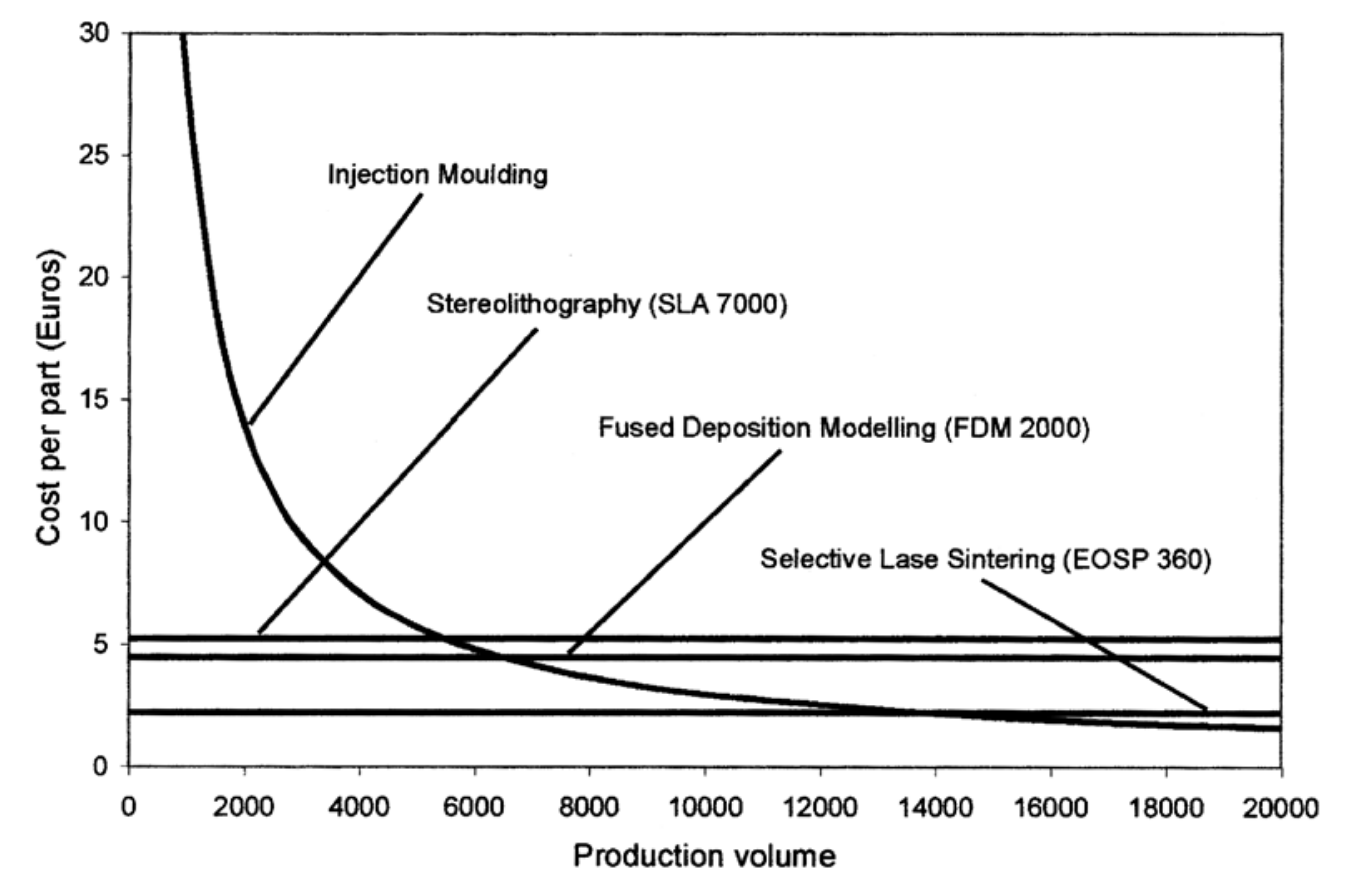
\includegraphics[width=0.55 \textwidth]{Images/costs.png}
    \caption[Traditional processes vs AM costs.]{Cost comparison for the manufacturing of a small plastic lever using different processes \cite{hopkinson_analysis_2003}.}
    \label{fig:costs}
\end{figure}
Furthermore, the initial machinery expenses were the primary cost factor in AM technologies. The authors believe these costs will decrease with mass adoption and technological advancements, thus reducing overall production costs. The real turning point for widely spread 3D printing occurred in the early 2010s, when patents for some polymers used in fused deposition modeling systems (FDM) expired. There was an absolute explosion of FDM 3D printer producers. We will discuss FDM shortly. Nowadays, additive manufacturing is employed in the production of small batches of finished products, sometimes even single-unit batches of highly customized products, or also in the prototyping phase.
These manufacturing processes do not intend to replace the traditional ones but rather allow us to expand the limits of what we can build. It is important to understand that additive manufacturing allows us to obtain components with mechanical functionalities and complexity unimaginable with traditional manufacturing processes but cannot be the only approach to production (at least for now).

%%%%%
%%%%%

% Additive Manufacturing Process Categories >>>
\section{Additive Manufacturing Process Categories} 
\label{sec:AMproc}
According to ISO/ASTM 52900 \cite{organization_isoastm_2015} and \citeauthor{gibson_additive_2015} (2015) there are seven different types of AM technologies: 
\begin{itemize}
    \item \textbf{Vat photo-polymerization processes} (VP). VP processes use radiation-curable resins or photopolymers that can be solidified using controlled light sources, usually ultraviolet radiation. Typically, it involves galvanometers to direct a laser beam or multiple directional light sources, such as controlled LEDs. The polymers used in this printing technology are usually acrylate-based or epoxy resins and industrial ceramic materials, such as alumina, zirconia, and silicon nitride. In recent years, new materials have been developed for the production of investment casting patterns \cite{3d_systems_investment_2023}, but also high technical performance material such as Cyanate Ester, which is used with Carbon Digital Light Synthesis\textsuperscript{TM} to produce pump turbines capable of withstanding high pressures (up to \numrange[range-phrase = --]{3800}{4000}\unit{\mega\pascal}) \cite{carbon_3d_carbon_2023}. The major advantages of this technology are the high level of accuracy of the finished products (up to \SI{0.05}{\milli\metre}), relatively high speed of manufacturing, and the variety of print sizes (ranging from tiny printers to larger ones, up to \qtyproduct{1000 x 800 x 500}{\milli\metre}. The disadvantages are that the finished prints require significant post-processing and that printers and the manufacturing process are still quite expensive. Moreover, material choices are limited to photopolymers only.
    \item \textbf{Fused filament fabrication} (FFF). FFF systems selectively extrude material as a filament through a heated nozzle. These processes are also called fused deposition modeling (FDM). These printers have a nozzle that is free to move in the horizontal plane and a system that moves it up and down along the z-axis (usually a threaded tube), allowing layer-wise material deposition. Typically employed materials are waxes, polyamide, acrylonitrile-butadiene-styrene, polyphenyl sulfone, polycarbonate, ceramics, and biocompatible or biodegradable materials. The main advantages of FFF systems include their widespread popularity and economic accessibility, as well as the variety of materials that can be used, such as ABS, which provides excellent structural properties, or PLA (polylactic acid), which can be extruded at relatively low temperatures and it is compostable. The drawbacks of this technology include lower print speeds and a lower achievable minimum resolution compared to other processes. We usually need to do some post-processing operations to achieve a satisfactory finishing.
    \item \textbf{Material jetting systems} (MJ). MJ is a technique that allows 3D printing of a piece using tiny droplets of liquid material selectively deposited onto a plate. Material jetting can be seen as the natural evolution of standard 2D inkjet printers but in three dimensions. MJ printers can use "cartridges" of materials and colors like traditional inkjet printers. One of the main advantages of MJ is the possibility of printing high-resolution multi-colored or multi-material objects. Initially, the materials used with this technology were waxes. Still, in recent years, the focus has been more on the deposition of acrylate photopolymers, in which droplets of materials are solidified with a UV lamp directly attached to the printing nozzle. The main advantages of MJ are the reduced material waste, as the deposition process is extremely precise (droplets of \numrange{25}{120} \unit{\micro\meter} at a rate of \numrange{0}{2000} \unit{drops / \second}), and the possibility of using different materials and colors simultaneously. The disadvantages of this solution are mostly the limited number of usable materials since only polymers and waxes or materials that are not excessively dense can be employed. Furthermore, the equipment required is relatively cheap, and the process can reach a remarkable printing speed.
    \item \textbf{Binder jetting systems}. Binder jetting is very similar to MJ. In binder jetting, a liquid binding agent called "binder" is selectively deposited in tiny droplets to solidify material powder, allowing different layers of powder to stick together. Due to the production method, the final objects may only sometimes be suitable for withstanding significant structural stresses and often require a long post-processing phase, which could increase variable costs. Binder jetting can be used with thermo-plastic polymers, metals, and ceramic materials. Compared to MJ, the significant advantages of this technology are the ability to use a much more vast range of materials and the higher printing speed. Moreover, it is possible to mix different powders to obtain final objects with specific mechanical features. However, printed parts often require a lot of post-processing work to improve the mechanical features and the finishing of the pieces.
    \item \textbf{Laminated object manufacturing} (LOM). In sheet lamination or laminated object manufacturing (LOM), layers of material are bonded together to form the final object. There are two possible approaches: "bond-then-form" and "form-then-bond." In the first case, the laminate is positioned and bonded to the substrate and then cut following the model contour. In the second case, the laminate material is cut, placed on the substrate, and bonded to the underlying layer. LOM techniques allow the usage of wood, thermo-plastic polymers, industrial ceramics, paper, polyvinyl chloride, and composite materials. The significant advantages of LOM are the ability to print large parts quickly and the lower equipment fixed costs compared to other types of AM processes.
    \item \textbf{Powder bed fusion} (PBF):  In these additive manufacturing techniques, a concentrated energy source is used to melt layers of powder selectively. Usually, the energy source is a laser (Selective Laser Sintering or SLS) or an electron beam (Electron Beam Melting or EBM), and the materials used can be polyamides, nylons, elastomers, and metals such as stainless steel, titanium, aluminum, cobalt, and copper. This AM technique is widely used for direct manufacturing and allows for producing finished objects with excellent mechanical properties and surface finishes.
    \item \textbf{Direct energy deposition} (DED): In DED, a concentrated heat energy source is used to melt material as soon as it is deposited selectively. Depending on the energy source used, we can further divide the processes into laser, electron beam, and plasma metal deposition. Moreover, depending on the shape of the material used, we can distinguish between powder-fed and wire-fed systems. Finally, depending on the direction in which the material is fed, we can distinguish between off-axis feeding, in which a side-mounted incident nozzle deposits the material, and coaxial feeding systems, in which the powder or wire material is deposited co-axially with the energy beam. The main advantage of DED is that it can be used to add parts to existing components or for repairs with a minimum need for support structures. There are several powders and printing area sizes available. However, DED has a lower accuracy compared to PBF, which makes DED unsuitable for producing complex shapes.
    \end{itemize}

% <<< End of Additive Manufacturing Process Categories

%%%%%
%%%%%

\section{Aim and Structure of the Work}
\label{sec:aimwork}
\begin{figure}
    \centering
    \subfloat[\label{fig:bugatti}]{
        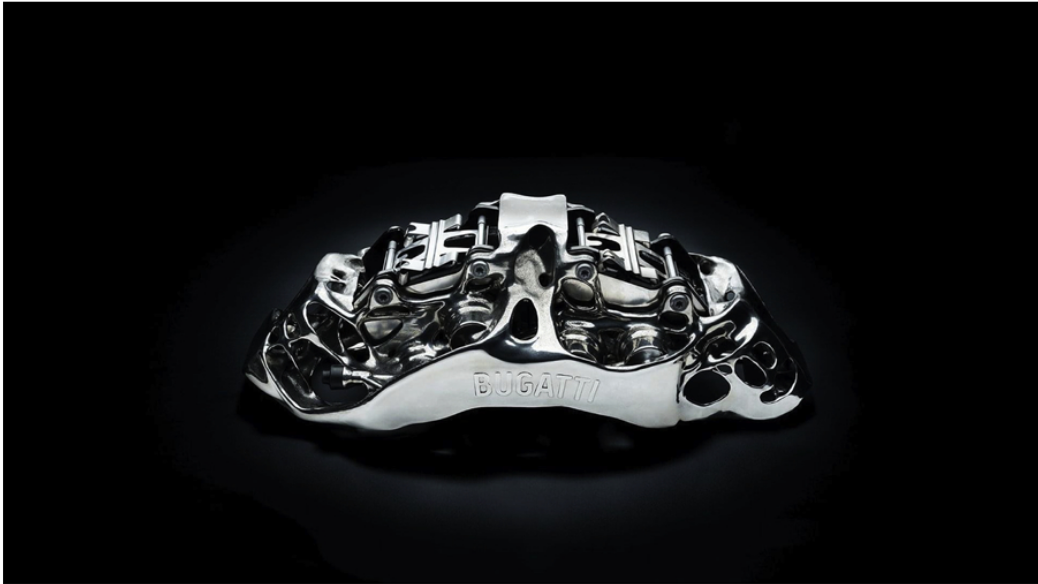
\includegraphics[scale=0.4]{Images/bugatti.png}
    }
    \quad
    \subfloat[\label{fig:supporto}]{
        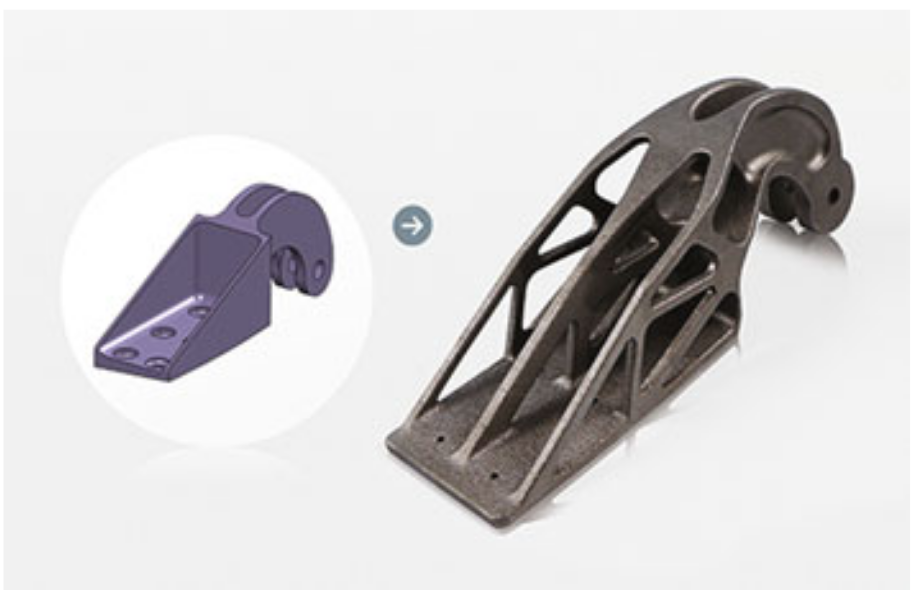
\includegraphics[scale=0.4]{Images/supporto.png}
    }
    \caption[Functional AM part printed in metal.]{On the left, a Bugatti brake caliper, one of the world’s largest functional parts produced in titanium alloy Ti6Al4V by AM. On the right, we can see support used in the aerospace industry. From \citeauthor{du_plessis_beautiful_2019}.}
    \label{fig:funcpart}
\end{figure}
In recent years, additive manufacturing processes for metallic parts, especially the so-called powder bed fusion processes, have revolutionized various industries, including aerospace, automotive, and energy. PBF processes are currently the most promising AM technology for printing structurally sound and functional components. Indeed, these processes are also used to create components that play a critical role during their use, often for safety reasons. Consider, for instance, the importance of the brake system shown in Fig. \ref{fig:bugatti}. Imagine the repercussions if the braking system failed on a Chiron that is speeding at \SI{350}{\kilo\metre /\hour}, or if aerospace support, like the one in Fig. \ref{fig:supporto}, may break, causing a \SI{8500}{\metre} fall of a heavy piece. For these reasons, as shown in Fig. \ref{fig:vchain}, the AM chain is particularly articulated, mainly due to the importance of the testing and certification phases. Data collected from process monitoring in AM presents a unique opportunity (compared to traditional manufacturing) for early defect detection or new non-destructive testing techniques.
\begin{figure}
    \centering
    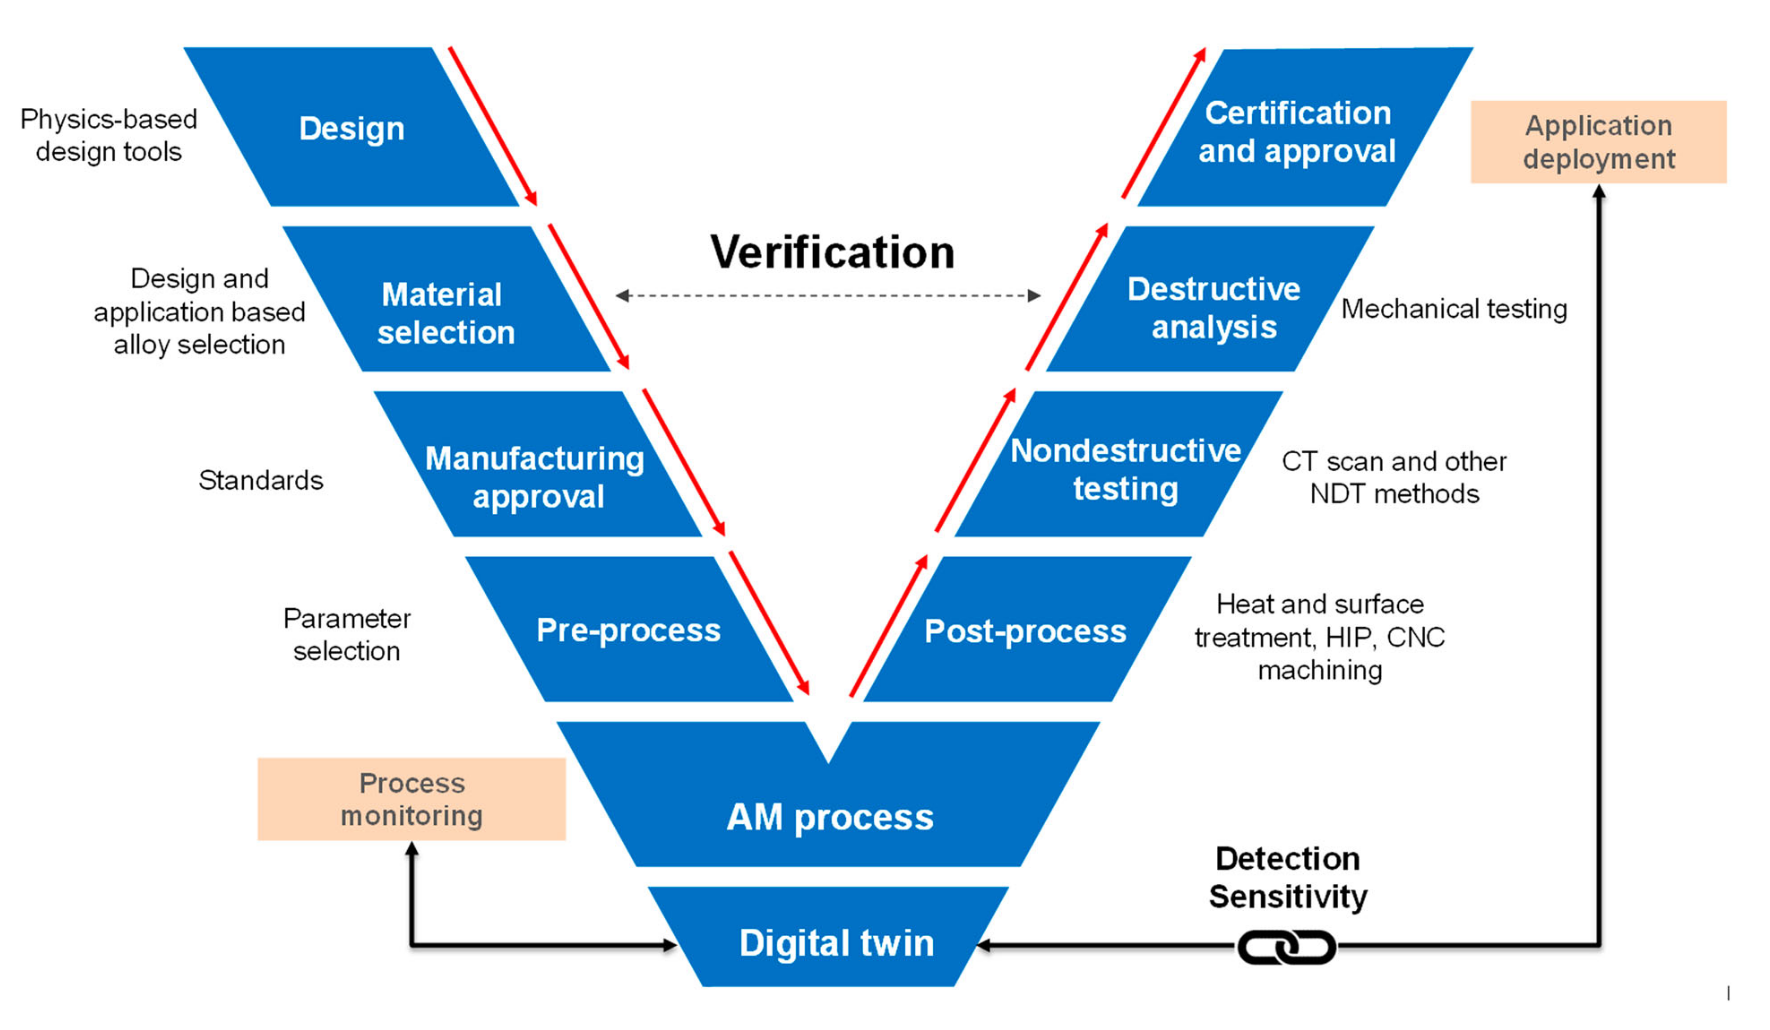
\includegraphics[width=0.65 \textwidth]{Images/v.png}
    \caption[AM process chain.]{V-shaped process chain for AM from design to certification \cite{moshiri_performance_2023}.}
    \label{fig:vchain}
\end{figure}
Quality control, defect detection, and ensuring the production process adheres to standards are crucial now more than ever. The temperature, particularly in additive manufacturing for metallic parts, significantly influences the mechanical properties of the finished product, as demonstrated in \citeauthor{williams_situ_2019} (2019). Indeed, the temperatures reach much higher peaks, and the cooling process is more dynamically complex. Anyone who has experience with "classical" FDM 3D printing for PLA would notice that the filament cools down in seconds. On the other hand, with metallic PBF printing, one must wait considerably longer before the final piece is extracted from the production chamber. Moreover, many additional factors could affect the temperature reached by the material during the PBF printing process and the consequent cooling process. This thesis aims to present a state-of-the-art review of identifying the so-called hot spots in PBF processes using machine learning algorithms. Hot spots are localized areas characterized by elevated temperatures for a sustained time and slower cooling drift, often attributable to their proximity to adjacent loose powder. The overheating leads to defects in the finished product.

This thesis is structured as follows. Chapter~\ref{ch:Metal_AM}, I will comprehensively describes PBF processes for 3D printing of metal parts, the necessary technologies, materials, and some potential applications. Chapter~\ref{ch:defects} outlines the most common defects in PBF processes, with a particular emphasis on the aforementioned hot spots, their causes, and the different monitoring systems used in AM. Chapter~\ref{ch:state_ot_the_art} is a literature review to present the state-of-the-art in hot spots detection using machine learning algorithms. The methods for the systematic review is explained in Appendix~\ref{ap:research}. Chapter~\ref{ch:baggingvoronoi} presents the bagging voronoi classification algorithm as an innovative approach that might lead to a deeper understanding of the hot spots phenomenon leveraging functional data, as well as providing a powerful non-destructive analysis tool for thermal profiles. Chapter~\ref{ch:conclusions} conclude the thesis and propose some research streams that could be explored further. Finally, Appendix~\ref{ap:Python}, proposes a simple Python \cite{python_software_foundation_python_2023} implementation of the algorithm proposed in Chapter~\ref{ch:baggingvoronoi}.